\documentclass[a4paper,12pt]{article}
\usepackage[utf8]{inputenc}
\usepackage{todonotes}
\usepackage[russian]{babel}
\usepackage{graphicx}
\usepackage{amsmath, amssymb}
\usepackage{hyperref}
\usepackage{float}
\usepackage{listings}
\usepackage{caption}
\usepackage{geometry}
\usepackage{xcolor}
\geometry{left=2cm,right=2cm,top=2cm,bottom=2cm}
\hypersetup{pdfborder=0 0 0}
\pagestyle{fancy}
\headsep=8mm
\footskip=20mm
\hypersetup{pdfstartview=FitH, linkcolor=linkcolor, urlcolor=urlcolor, colorlinks=true}

\definecolor{strings}{rgb}{0,0.6,0}
\definecolor{comments}{rgb}{0,0.3,0}
\definecolor{numbers}{rgb}{0.5,0.5,0.5}
\definecolor{keywords}{rgb}{0.09,0.61,0.95}
\definecolor{background}{rgb}{0.97,0.97,0.97}

\lstdefinestyle{codestyle}{
    backgroundcolor=\color{background},
    commentstyle=\color{comments},
    keywordstyle=\color{keywords},
    stringstyle=\color{strings},
    numberstyle=\tiny\color{numbers},
    basicstyle=\ttfamily\scriptsize,
    breakatwhitespace=false,
    breaklines=true,
    captionpos=b,
    inputencoding=utf8,
    keepspaces=false,
    numbers=left,
    numbersep=5pt,
    showspaces=false,
    showstringspaces=false,
    showtabs=false,
    tabsize=2,
    extendedchars=true
}

\lstset{style=codestyle}

\begin{document}

% Титульный лист
\begin{titlepage}
    \centering
    {\large Федеральное государственное автономное образовательное учреждение\par}
    {\large высшего образования\par}
    {\bfseries САНКТ-ПЕТЕРБУРГСКИЙ НАЦИОНАЛЬНЫЙ ИССЛЕДОВАТЕЛЬСКИЙ УНИВЕРСИТЕТ ИТМО\par}
    {\bfseries Факультет систем управления и робототехники\par}
    \vfill
    {\Large \bfseries Лабораторная работа №1\par}
    {\Large \bfseries Гистограммы, профили и проекции\par}
    \vfill
    
    \begin{flushright}
        Студенты: & Бахтаиров Р.А.,\\ Сайфуллин Д.Р. \\
        Поток: & Тех.Зр R23 1.1 \\
        Преподаватель: & Шаветов С.В.
    \end{flushright}
    \vfill
    Санкт-Петербург, 2025 г.
\end{titlepage}

% Оглавление
\tableofcontents
\newpage

% Введение
\section{Цель работы}
В этой работе мы изучим основные яркостные и геометрические характеристики изображений для их анализа.
\section{Изображение, которое будем использовать для проверки функций}
\begin{figure}[H]
    \centering
    \includegraphics[width=0.8\textwidth]{images/test.png}
    \label{fig:profile}
\end{figure}


% Основной код
\section{Изначальный код работы}
Часть кода будет приведена ниже с указанием необходимых импортов, вычислением гистограмм и их отрисовкой. Остальная часть будет приведена в файле, приложенном к отчёту.
\subsection{Необходимые импорты}
\begin{lstlisting}[language=Python, caption=Импорт библиотек]
import cv2 as cv
import numpy as np
import matplotlib.pyplot as plt
import sys
\end{lstlisting}
В данной работе используются несколько библиотек для обработки изображений, вычислений и визуализации.
\begin{itemize}
    \item Библиотека \verb|OpenCV| предназначена для обработки изображений и задач компьютерного зрения.
    \item \verb|NumPy| - библиотека для работы с многомерными массивами и выполнения математических вычислений.
    \item \verb|Matplotlib|, а именно её модуль Pyplot, используется для визуализации данных.
\end{itemize}

\subsection{Отрисовка гистограмм для чёрно-белых изображений}
\begin{lstlisting}[language=Python, caption=Вычисление нормализованных RGB- и кумулятивных гистограмм]
def DrawHist(image, data_array, color, max_val = 1.0):
  image_w = image.shape[1]
  image_h = image.shape[0]
  data_size = data_array.shape[0]

  step = image_w / data_size
  x = 0
  for i in range(0, data_size):
    cv.rectangle(image,
                 (int(x), image_h - 1 - int((image_h - 1) * data_array[i] / max_val)),
                 (int(x + step) - 1, image_h - 1),
                 color, thickness = -1)
    x += step

def DrawGraph(image, data_array, color, max_val = 1.0):
  image_w = image.shape[1]
  image_h = image.shape[0]
  data_size = data_array.shape[0]

  step = image_w / data_size
  x = step * 0.5
  cv.line(image,
          (0, image_h - 1 - int((image_h - 1) * data_array[0] / max_val)),
          (int(x), image_h - 1 - int((image_h - 1) * data_array[0] / max_val)),
          color, thickness = 1)

  for i in range(1, data_size):
    cv.line(image,
            (int(x), image_h - 1 - int((image_h - 1) * data_array[i - 1] / max_val)),
            (int(x + step), image_h - 1 - int((image_h - 1) * data_array[i] / max_val)),
            color, thickness = 1)
    x += step

  cv.line(image,
          (int(x), image_h - 1 - int((image_h - 1) * data_array[data_size - 1] / max_val)),
          (image_w - 1, image_h - 1 - int((image_h - 1) * data_array[data_size - 1] / max_val)),
          color, thickness = 1)
\end{lstlisting}

Функция \texttt{DrawHist} предназначена для отрисовки столбчатой гистограммы на заданном изображении. Гистограмма рисуется в виде прямоугольников, высота которых соответствует нормализованным значениям входных данных.

Функция \texttt{DrawGraph} выполняет аналогичную задачу, но вместо столбцов использует линии, соединяющие последовательные точки данных. Это позволяет визуализировать изменения значений более плавно по сравнению со столбчатой гистограммой. Также, при отрисовки более одной гистограммы, позволяет избежать возможных ошибок отображения. 

Обе функции используются для наглядного представления распределения яркости в изображении, 
что помогает анализировать его характеристики и применять различные методы обработки.

\subsection{Отрисовка гистограмм для цветных изображений}
\begin{lstlisting}[language=Python, caption=Отрисовка RGB- и кумулятивной гистограмм]
def SimpleHistogram(I):
  if I.ndim == 2:
    hist = cv.calcHist([I], [0], None, [256], [0, 256])[:, 0]

    hist_img = np.full((256, 512, 3), 255, dtype = np.uint8)
    
    DrawHist(hist_img, hist, (127, 127, 127), hist.max())
  else:
    bgr_planes = cv.split(I)

    hist_b = cv.calcHist(bgr_planes, [0], None, [256], [0, 256])[:, 0]
    hist_g = cv.calcHist(bgr_planes, [1], None, [256], [0, 256])[:, 0]
    hist_r = cv.calcHist(bgr_planes, [2], None, [256], [0, 256])[:, 0]

    hist_img = np.full((256, 512, 3), 255, dtype = np.uint8)
    hist_scale = np.max([hist_b.max(), hist_g.max(), hist_r.max()])
    DrawGraph(hist_img, hist_b, (255, 0, 0), hist_scale)
    DrawGraph(hist_img, hist_g, (0, 255, 0), hist_scale)
    DrawGraph(hist_img, hist_r, (0, 0, 255), hist_scale)

  return hist_img
\end{lstlisting}


Функция \texttt{SimpleHistogram} предназначена для построения гистограммы изображения и её визуализации.
Если входное изображение является градациями серого (чёрно-белым), функция вычисляет его гистограмму, используя метод \texttt{cv.calcHist}, а затем визуализирует её с помощью функции \texttt{DrawHist}.

Если изображение цветное, оно разбивается на три канала (синий, зелёный и красный) с помощью функции \texttt{cv.split}. Затем для каждого канала рассчитывается отдельная гистограмма, после чего она визуализируется с использованием функции \texttt{DrawGraph} в соответствующем цвете (синий, зелёный, красный).
\subsection{Отрисовка кумулятивной гистограммы}
\begin{lstlisting}[language = Python, caption = Кумулятивная гистограмма для чб изображения]
def Histogram(I):
  if I.ndim != 2:
    return None
  hist = cv.calcHist([I], [0], None, [256], [0, 256])[:, 0]
  cum_hist = np.cumsum(hist) / I.shape[0] / I.shape[1]
  hist_img = np.full((256, 512, 3), 255, dtype = np.uint8)
  DrawHist(hist_img, hist, (127, 127, 127), hist.max())
  DrawGraph(hist_img, cum_hist, (0, 0, 0), 1)
  
  return hist_img
\end{lstlisting}
И функция \verb|SimpleHistogram_with_cumulation|, которая возвращает гистограмму и кумулятивную гистограмму как для чёрно-белого, так и цветного изображения
\begin{lstlisting}[language = Python, caption = Функция для отрисовки гистограммы и кумулятивной гистограммы для цветного изображения]
def SimpleHistogram_with_cumulation(I):
  if I.ndim == 2:
    return Histogram(I)
  else:
    # Split an image into layers and work with them separately
    bgr_planes = cv.split(I)
    # Calculate histogram
    hist_b = cv.calcHist(bgr_planes, [0], None, [256], [0, 256])[:, 0]
    hist_g = cv.calcHist(bgr_planes, [1], None, [256], [0, 256])[:, 0]
    hist_r = cv.calcHist(bgr_planes, [2], None, [256], [0, 256])[:, 0]
    # Draw histogram
    hist_img = np.full((256, 512, 3), 255, dtype = np.uint8)
    hist_scale = np.max([hist_b.max(), hist_g.max(), hist_r.max()])
    #Calculate sum histogram
    B_cum_hist = np.cumsum(hist_b) / I[0].shape[0] / I[0].shape[1]
    G_cum_hist = np.cumsum(hist_g) / I[1].shape[0] / I[1].shape[1]
    R_cum_hist = np.cumsum(hist_r) / I[2].shape[0] / I[2].shape[1]
    #Norming the cumulate_hist
    koeff_of = hist_scale/B_cum_hist.max()
    B_cum_hist, G_cum_hist,R_cum_hist= [i*koeff_of for i in (B_cum_hist, G_cum_hist,R_cum_hist)]
    DrawGraph(hist_img, hist_b, (255, 0, 0), hist_scale)
    DrawGraph(hist_img, B_cum_hist, (255, 0, 0), hist_scale)
    DrawGraph(hist_img, hist_g, (0, 255, 0), hist_scale)
    DrawGraph(hist_img, G_cum_hist, (0, 255, 0), hist_scale)
    DrawGraph(hist_img, hist_r, (0, 0, 255), hist_scale)
    DrawGraph(hist_img, R_cum_hist, (0, 0, 255), hist_scale)
  return hist_img    
\end{lstlisting}
Ниже представлен наглядный пример работы этих функций(как для чёрно-белого изображения, так и для цветного)
\begin{figure}[H]
    \begin{minipage}{0.5\textwidth}
        \centering 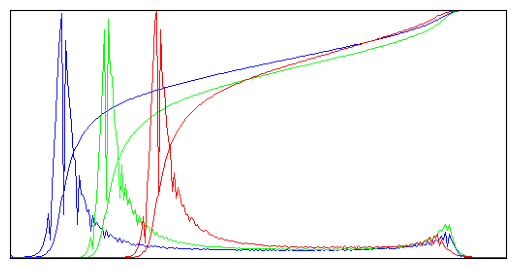
\includegraphics[width=\textwidth]{images/col_hist.png}
    \end{minipage}\hfill
    \begin{minipage}{0.5\textwidth}
        \centering 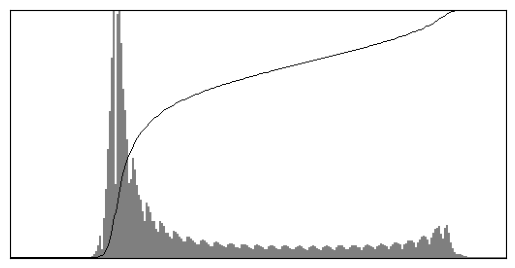
\includegraphics[width=\textwidth]{images/bw_hist.png}
    \end{minipage}
    \caption{Гистограмма и кумулятивная гистограмма для цветного и чёрно-белого изображений}
\end{figure}

\section{Методы преобразования изображений}
В этом разделе описаны методы преобразования изображений, используемые в лабораторной работе.
\begin{enumerate}
    \item  Shift(смещение)
    \item  Linear transformation(линейная транформация)
    \item  Linear equalization(линейное выравнивание)
    \item  Nonlinear dynamic range stretching(нелинейное динамическое растяжение диапазона)
    \item Uniform transformation(равномерное распределение)
    \item  Exponential transformation(экспоненциальное преобразование)
    \item  Rayleigh transformation(преобразование Рэлея)
     \item 2/3 degree transformation(преобразование степени 2/3)
     \item Hyperbolic transformation(Гиперболическая трансформация)
\end{enumerate}
\subsection{Shift}
Идея этого метода заключается в том, чтобы прибавить к значению интенсивности каждого пикселя некоторое значение \texttt{val}. В результате гистограмма изображение сместится на \texttt{val}, от чего метод и получил своё название. Тем не менее, в ходе выполнения данного метода мы можем для выйти за границы допустимых значений интенсивности $I$. Для для того, чтобы избежать ошибки мы выполняем опрерацию \verb|np.clip(image, min_val, max_val)|. В математической форме операция выглядит таким образом:
$$I_{shift}[x](val) = \begin{cases}
   0          &\text{if } I[x] + val < 0 \\
   I[x] + val &\text{if } 0 <= I[x] + val <= 255 \\
   255        &\text{if } I[x] + val > 255
\end{cases}$$
\begin{figure}[H]
    \centering 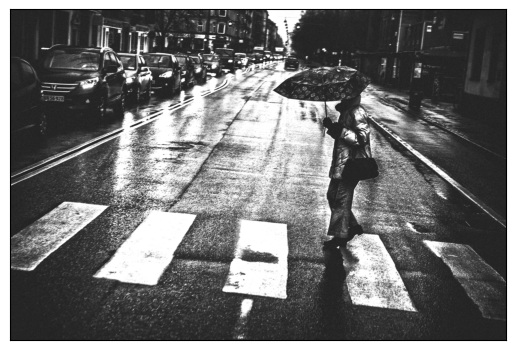
\includegraphics[width=0.7\textwidth]{images/shift.png}
    \caption{Применение смещения}
    \centering 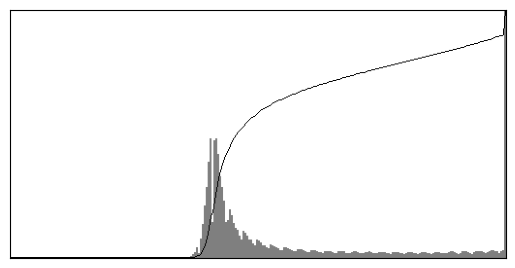
\includegraphics[width=0.7\textwidth]{images/shift_hist.png}
    \caption{Гистограмма после применения метода}
\end{figure}
\subsection*{Предисловие к следующим методам}
Далее, для преобразования изображений мы будем использовать \verb|LUT|. \verb|LUT| - эта функция(таблица значений), которая применяется на значение интенсивности пикселя и заменяет его на некоторое другое. 
$LUT(x_i)= y_i$ - где $x_i$ - значение интенсивности, а $y_i$ - новое значение. \verb|LUT| применяется сразу на все пиксели с одинаковым значением $x_i$. 
Функция $P(x)$ - куммулятивная функция для значения интенсивности $x$
$I,I\_min, I\_max$ - значения интенсивностей(нынешней, минимальной и максимальной соответсвенно)

\subsection{Linear equalization}
Арифметическая запись метода:
$$LUT(x) = P(x) \cdot 255$$
Данный метод меняет значение интенсивности $x$ на значение кумулятивной функции(гистограммы). Для перехода с интервала $[0,1]$ к интервалу $[0,255]$ производится домножение на 255. В результате кумулятивная гистограмма нового распределения интенсивности пикселей будет линейной. Так как кумулятивная функция не является ''дискретно непрерывной'' , то есть возможны значения $\{1,2,5,10\ldots\}$, то и в гистограмме нового распределения интенсивности возможны разрывы. Это можно пронаблюдать на примере снизу.
\begin{figure}[H]
    \centering 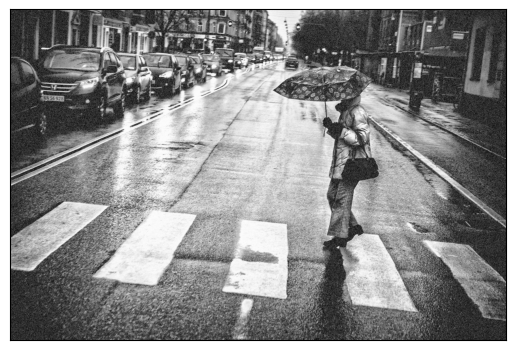
\includegraphics[width=0.7\textwidth]{images/linear.png}
    \caption{Применение линейного выравнивания}
    \centering 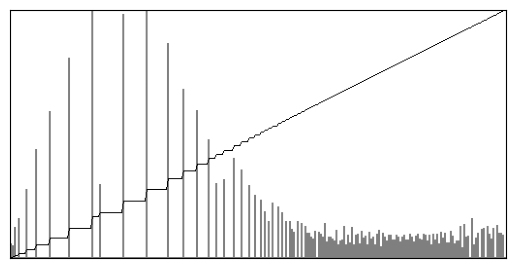
\includegraphics[width=0.7\textwidth]{images/linear_hist.png}
    \caption{Гистограмма после применения метода}
\end{figure}
\subsection{Nonlinear dynamic range stretching}
Арифметическая запись метода:
$$lut_{[0,255]}(x) = \left( \dfrac{x - I_{min}}{I_{max} - I_{min}} \right) ^ \alpha \cdot 255$$
В данном методе происходить нормировка значений интенсивности в интервал $[0,1]$, а после возводится в степень $\alpha$. В результате, если $\alpha$ было больше 1, то большие значения интенсивности так и останутся большие, а маленькие окажутся значительно меньше: $0.99^2 = 0.98,  0.1^2 = 0.01$. В зависимости от $\alpha$ мы можем контролировать какие именно значения будут уменьшаться, а какие увеличиваться.
\begin{figure}[H]
    \centering 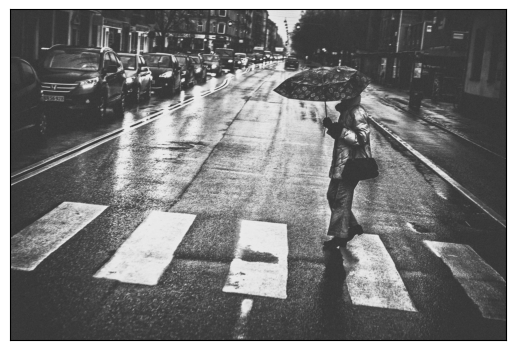
\includegraphics[width=0.7\textwidth]{images/nonlin.png}
    \caption{Применение нелинейного динамического растяжения диапазона}
    \centering 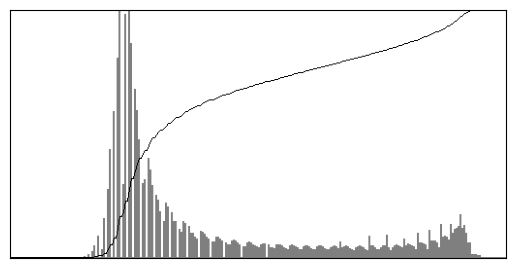
\includegraphics[width=0.7\textwidth]{images/nonlin_hist.png}
    \caption{Гистограмма после применения метода}
\end{figure}

\subsection{Uniform transformation}
Арифметическое представление:
$$LUT(x) = (I_{max} - I_{min}) \cdot P(x) + I_{min}$$
Данное трансформация изображения очень похоже на \texttt{Linear equalization}, но имеет важные отличия, если $I\_min \neq 0$  и  $I\_max \neq 255$. В этом случае "линейная" нормировка будет проведена не на всю прямую $[0,255]$, а лишь на отрезок $[I\_min, I\_max]$.
\begin{figure}[H]
    \centering 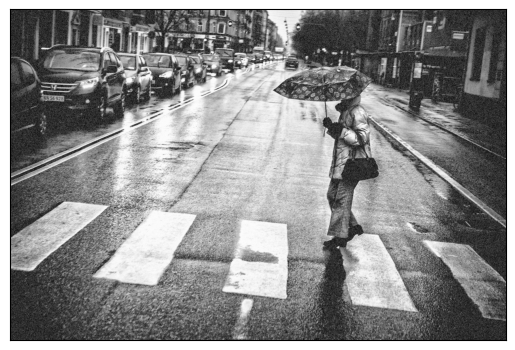
\includegraphics[width=0.7\textwidth]{images/uniform.png}
    \caption{Применение равномерного распределения}
    \centering 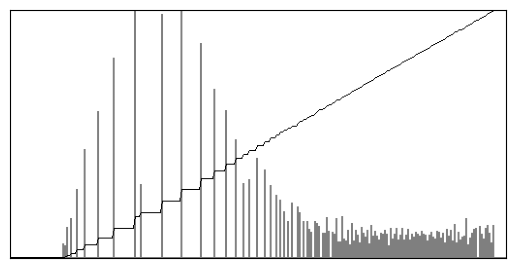
\includegraphics[width=0.7\textwidth]{images/uniform_hist.png}
    \caption{Гистограмма после применения метода}
\end{figure}

\subsection{Exponential transformation}
Арифметическое представление преобразования:
$$LUT_{[0,255]}(x) = \left( \dfrac{I_{min}}{255.0} - \dfrac{1}{\alpha} \cdot \ln\left(1-P(x)\right) \right) \cdot 255$$
Где коэффициент $\alpha$ определяется нами. 
Как видно ниже, из-за того, что построение этого распределения было основано на функции $P$ в гистограмме нового распределения есть пробелы. 
С ростом значения куммулятивной функции(а соответственно и значения интенсивности) логарифм вносит всё большее влияние в функцию. Такое свойство функции выражается на гистограмме в значительном росте "шага" между значениями, при значениях, приближающихся к максимуму.
\begin{figure}[H]
    \centering 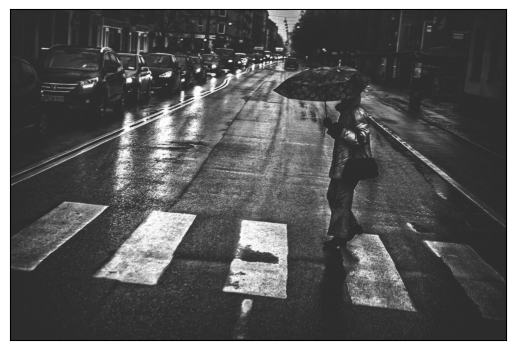
\includegraphics[width=0.7\textwidth]{images/exp.png}
    \caption{Применение экспоненциального преобразования}
    \centering 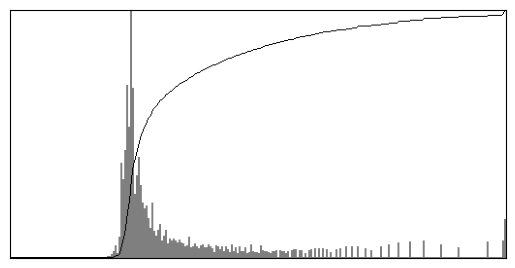
\includegraphics[width=0.7\textwidth]{images/exp_hist.png}
    \caption{Гистограмма после применения метода}
\end{figure}

\subsection{Rayleigh transformation}
Арифметическое представление трансформации:
$$LUT_{[0,255]}(x) = \left(\dfrac{I_{min}}{255.0}+\sqrt{2\alpha^2 \ln\left(\dfrac1{1-P(x)}\right)}\right) \cdot 255$$
Опять же, параметр $\alpha$ мы выбираем сами. Распределение Рэлея является распределением, проистекающим из теории вероятности. График его имеет значительное уплотнее в центре и растяжение по левому и правому краю. Такое свойство этой функции можно увидет на гистограмме.
\begin{figure}[H]
    \centering 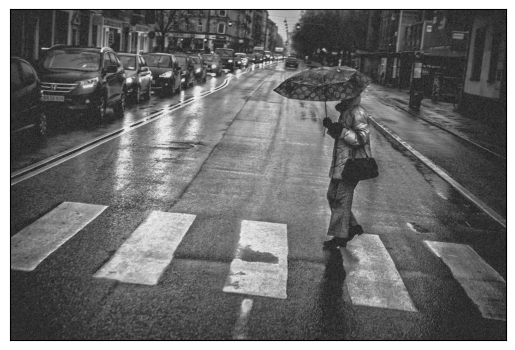
\includegraphics[width=0.7\textwidth]{images/ray.png}
    \caption{Применение преобразования Рэлея}
    \centering 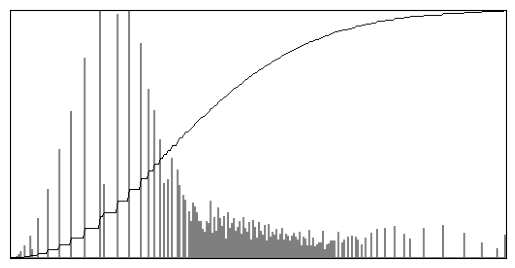
\includegraphics[width=0.7\textwidth]{images/ray_hist.png}
    \caption{Гистограмма после применения метода}
\end{figure}

\subsection{2/3 degree transformation}
Арифметическое представление:
$$LUT_{[0,255]}(x) = P(x)^{2/3} \cdot 255$$
Эта трансформация изображения обладает довольно интересным свойством. Так как область значения кумулятивной функции это отрезок $[0,1]$, то при возведение в степень  2/3 все пиксели, значения которых приближены к белым остаются белыми, а серые и черные наоборот, становятся ещё чернее.Тем не менее, данное преобразование больше склонно к высветление изображения.

\begin{figure}[H]
    \centering 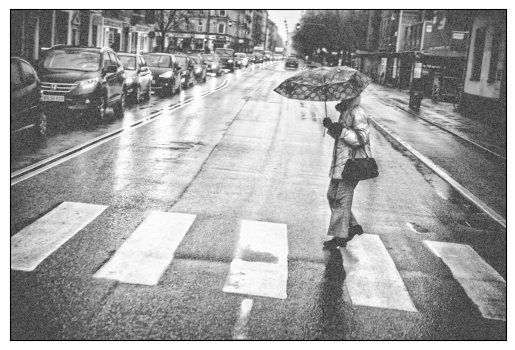
\includegraphics[width=0.7\textwidth]{images/23.png}
    \caption{Применение преобразования степени 2/3}
    \centering 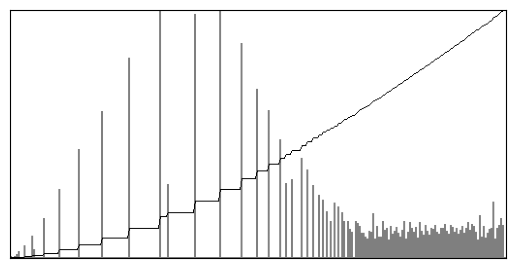
\includegraphics[width=0.7\textwidth]{images/23_hist.png}
    \caption{Гистограмма после применения метода}
\end{figure}

\subsection{Hyperbolic transformation}
Арифметическое представление:
$$LUT_{[0,255]}(x) = \alpha^{P(x)} \cdot 255$$
Стоит понимать, что в данном распределение необходимо взять $\alpha$ меньшее единицы(и большее 0). Обычно за $\alpha$ берум минимальное значение кумулятивной функции или интенсивности. Данное распределение ведеёт себя как показательная функция на отрезке $[0,1]$, то есть с ростом $I$ будет убывать, а максимума достигает при $I=0$. В итоге интенсивность на картинке инвертируется 

\begin{figure}[H]
    \centering 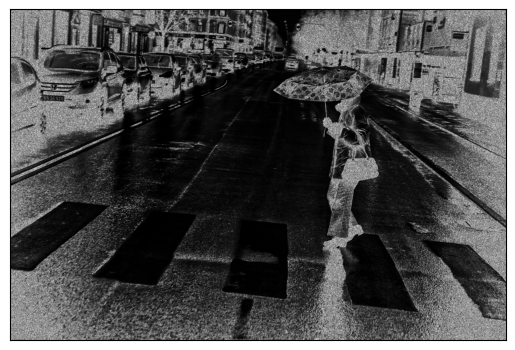
\includegraphics[width=0.7\textwidth]{images/hyp.png}
    \caption{Применение гиперболической трансформации}
    \centering 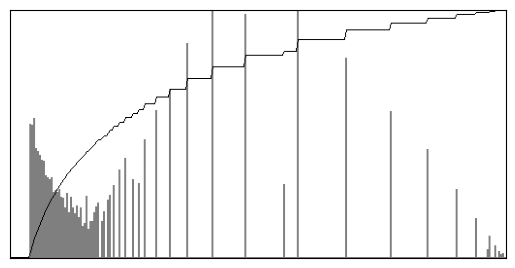
\includegraphics[width=0.7\textwidth]{images/hyp_hist.png}
    \caption{Гистограмма после применения метода}
\end{figure}

\section{Профили изображений}
Профиль изображения вдоль заданной линии представляет собой одномерную функцию интенсивности, полученную из двумерного изображения путем выделения значений яркости вдоль определенной траектории. Этот метод анализа широко используется в обработке изображений для исследования структуры и свойств объектов.

В данном задании необходимо выполнить анализ профиля изображения, содержащего объект с выраженными контрастными границами --- штрих-код. Выполнение задания включает в себя следующие этапы:
\begin{enumerate}
    \item Загрузка изображения в градациях серого для упрощения анализа яркости.
    \item Выбор линии, вдоль которой будет построен профиль (например, центральная горизонтальная линия изображения).
    \item Извлечение значений интенсивности пикселей вдоль выбранной линии.
    \item Очистка данных профиля, устранение шумов и сглаживание графика.
    \item Анализ полученного профиля: выявление закономерностей, обнаружение резких переходов в яркости.
    \item Приведение результатов к удобному виду для дальнейшего анализа.
    \item Графическое представление профиля для визуального анализа.
\end{enumerate}
\begin{figure}[H]
    \centering
    
\includegraphics[width=0.7\textwidth]{images/barcode.png}
    \caption{Исходное изображение}
    \label{fig:profile}
    \centering
    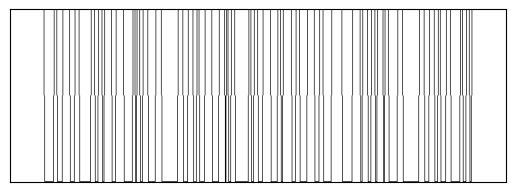
\includegraphics[width=0.7\textwidth]{images/code.png}
    \caption{Профиль яркости}
    \label{fig:profile}
\end{figure}

После выполнения эксперимента можно увидеть, что профиль изображения отражает структуру его интенсивности вдоль заданного направления. В случае анализа штрих-кода, профиль демонстрирует характерные чередующиеся пики и спады, соответствующие черным и белым полосам. Это подтверждает полезность профилей для задач анализа контуров и сегментации изображений. Дополнительно, применение фильтрации и сглаживания профиля позволяет исключить шумовые помехи и сделать анализ более точным.

\section{Проекции изображений}

Проекция изображения — это способ упростить его анализ. Она показывает, как распределена яркость в изображении, суммируя значения пикселей в одном направлении. Это помогает находить границы объектов и анализировать их расположение.

Есть два вида проекций: горизонтальная и вертикальная. Горизонтальная проекция складывает яркости пикселей по строкам, а вертикальная — по столбцам. Они используются в распознавании текста, анализе штрих-кодов и выделении объектов на изображении.

\begin{figure}[H]
    \begin{minipage}{0.5\textwidth}
        \centering 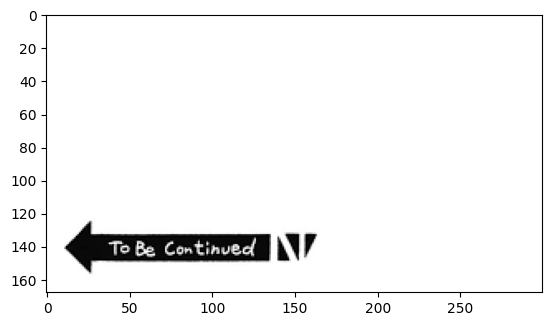
\includegraphics[width=\textwidth]{images/im.png}
        \caption{Исходное изображение}
    \end{minipage}
    \begin{minipage}{0.4\textwidth}
        \centering 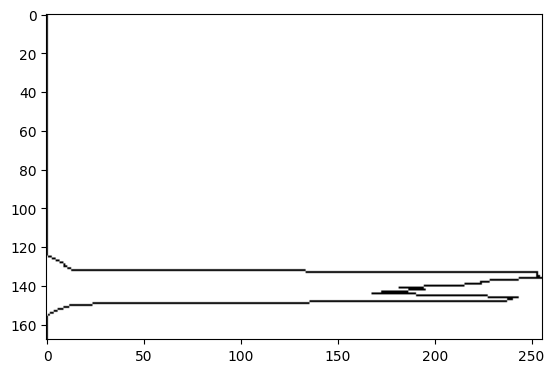
\includegraphics[width=\textwidth]{images/im_pr_y.png}
        \caption{Проекция на Y}
    \end{minipage}\\
    \begin{minipage}{0.5\textwidth}
        \centering 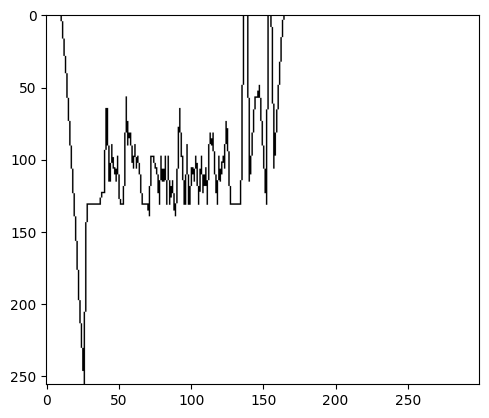
\includegraphics[width=\textwidth]{images/im_pr_x.png}
        \caption{Проекция на X}
    \end{minipage}\hfill
    \begin{minipage}{0.5\textwidth}
        \centering 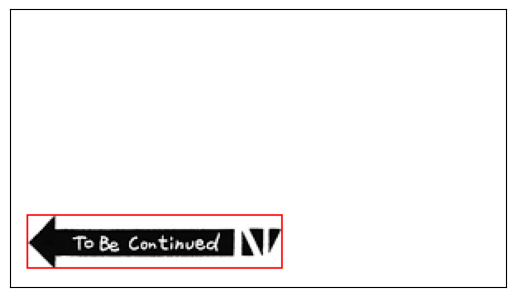
\includegraphics[width=\textwidth]{images/im_bound.png}
        \caption{Баунд по найденным проекциям}
    \end{minipage}
\end{figure}\noindent

Эксперимент показал, что метод проекций хорошо помогает находить границы объектов. Это удобно для компьютерного зрения, когда нужно автоматически выделять важные элементы на изображении. Однако он работает лучше всего на картинках с четкими границами. Если изображение сложное или содержит шум, потребуется дополнительная обработка.

% Результаты
\section{Результаты}
В этой лабораторной работе мы освоили методы преобразования изображения для изменения его характеристик и улучшения визуального качества, чтобы в последующем упростить анализ изображения. Кроме того, мы изучили профили и проекции изображения, которые также помогают в анализе изображения и благодаря которым мы сможем выделять границы и объекты на изображении. К тому же мы познакомились с библиотекой \verb|OpenCV| и библиотекой \verb|Matplotlib|, которые упрощают работу с изображениями и визуализацией результаты --- всё это помогло нам лучше понять, как работают представленные преобразования.

\section{Вопросы к защите}
\begin{enumerate}
    \item Что такое контрастность изображения и как её можно изменить?\\[0.5em]
    Контрастность изображения --- это интервал между самым тёмным и самым ярким пикселем изображения. Её можно изменить с помощью различных преобразований, выбрав наиболее подходящие для конкретного изображения.
    \item Чем эффективно использование профилей и проекций изображения?\\[0.5em]
    Профили и проекции изображения помогают в определении границ и размеров объектов на монотонном изображении, а также в анализе шаблонов и обрезании изображений.
    \item Каким образом можно найти объект на равномерном фоне?\\[0.5em]
    Можно использовать проекции изображения на одну из осей, чтобы найти расположение объектов, а затем с помощью профилей определить форму и границы объекта на двумерной плоскости, чтобы выделить его.
\end{enumerate}

\end{document}
